\chapter{Background} \label{background}

\bigskip \bigskip The thesis work precisely incorporates around the topic of industrial risk assessments and how knowledge modeling can be of use in that area. 

\section{Industrial risk assessment} \label{ira}
If risk cannot be managed, it cannot be controlled and if it cannot be controlled it cannot be managed as stated by Korenko et al. \cite{Korenko}. Industrial risk assessment is the process of identifying potential hazards and assessing the associated risks in industrial settings. The goal of industrial risk assessment is to improve safety and prevent accidents in the workplace by identifying potential hazards and implementing appropriate mitigation strategies. 

\paragraph{} Industrial risk assessment involves several steps, including hazard identification, risk assessment, and risk management. In the hazard identification step, potential hazards in the industrial system are identified. This can involve a review of the equipment, processes, and materials used in the industrial system. In the risk assessment step, the likelihood and consequences of each identified hazard are assessed. This involves quantifying the likelihood of the hazard occurring and the severity of the consequences should it occur. Shah et al. discussed that the risk assessment process can involve mathematical modeling, simulation, and expert judgment \cite{LAShah}. In the risk management step, appropriate mitigation strategies are identified and implemented to reduce the likelihood of the hazard occurring or mitigate the consequences should it occur. Mitigation strategies can include engineering controls, administrative controls, and personal protective equipment.

\paragraph{} Industrial risk assessment is essential for ensuring the safety of workers and preventing accidents in industrial settings. Industrial accidents can have severe consequences, including injuries, fatalities, and damage to equipment and facilities. By identifying potential hazards and implementing appropriate mitigation strategies, organizations can reduce the likelihood of accidents and improve safety in the workplace. Also, compliance with industrial safety regulations is essential to ensure the safety of workers and prevent accidents. Industrial risk assessment can help organizations comply with safety regulations by providing insights into potential hazards and effective mitigation strategies (Peron et al. \cite{https://doi.org/10.1111/risa.14010}).

\subsection{Safety standards} \label{standards}
Safety standards are written documents that are guidelines or requirements established by regulatory bodies or professional organizations that aim to ensure the safety of workers and prevent accidents in industrial settings. Safety standards are designed to provide a framework for identifying and addressing potential hazards and implementing appropriate mitigation strategies.

\paragraph{} In industrial risk assessments, compliance with safety standards is essential to ensure the safety of workers and prevent accidents in the workplace. Industrial safety standards cover various aspects of safety, including equipment safety, process safety, electrical safety, and personal protective equipment (PPE) safety, as discussed by Korenko et al. \cite{Korenko}. For example, safety standards may require the use of specific safety equipment or the implementation of safety procedures to prevent accidents related to machinery operation. Therefore, the safety standards contains a wide array of requirements for the risk assessments. 

\paragraph{} In industrial risk assessments, safety standards can be used as a reference point for identifying potential hazards and determining appropriate mitigation strategies. Safety standards can provide insights into the types of hazards that are common in a particular industry or process and the recommended mitigation strategies to reduce the associated risks. Additionally, compliance with safety standards can help organizations avoid legal liability and regulatory fines resulting from accidents or failure to comply with safety regulations \cite{Pacaiova}.

\paragraph{} According to the International Organization for Standardization (ISO) \cite{ISO12100}, there are three categories of standards,
\begin{itemize}
    \item Type A standards, also known as basic safety standards, are fundamental standards that provide general requirements for safety and basic concepts, principles, and terminology applicable to all products. They are intended to be applied in conjunction with other product-specific standards.
    \item Type B standards, also known as group safety standards, provide detailed safety requirements for specific types of products or product families. They cover the specific hazards associated with the product or product family and provide detailed guidance on how to mitigate those hazards.
    \item Type C standards, also known as particular safety standards, provide specific safety requirements for individual products or product models. They are intended to supplement Type A and Type B standards and provide detailed guidance on how to ensure the safety of a specific product or model.
\end{itemize}

\subsection{ISO 12100} \label{iso12100}
The thesis is based on the international standard ISO 12100 \cite{ISO12100}. This standard is chosen since it is a Type A standard, therefore it is a fundamental standard that provide general requirements for safety applicable to multiple products. Also it is scalable, if we look at it from the knowledge modeling perspective, since it refers to multiple standards and can also direct towards more specific Type C standards when implementing on a specific product. ISO 12100 is an international standard that provides guidelines for the design and implementation of machinery safety. The standard outlines a risk assessment and risk reduction process for machinery designers and manufacturers to follow in order to reduce the risk of injury to workers who use or maintain machinery.

\paragraph{} The standard is divided into three parts:
\begin{enumerate}
    \item Part 1: General Principles for Design - This section provides an overview of the risk assessment and risk reduction process and provides general principles for machinery design to ensure safety.
    \item Part 2: Technical Principles - This section provides technical guidance for machinery design and risk reduction. It covers specific hazards and provides guidance on how to address them.
    \item Part 3: Documentation and Verification - This section provides guidance on documentation requirements for machinery safety and verification methods to ensure compliance with safety requirements.
\end{enumerate}

\paragraph{} The ISO 12100 standard is widely recognized and accepted in many countries around the world. Compliance with the standard can help machinery designers and manufacturers ensure that their machinery is safe and compliant with international safety requirements.

\subsection{Industrial risk assessment in a TIC company}

A TIC company is a company that provides testing, inspection, and certification services for various products, services, or processes. TIC companies help their clients to ensure the safety, quality, and performance of their offerings and to comply with the relevant standards and regulations. Testing services typically involve evaluating the performance, quality, and safety of products or materials through various testing procedures. Inspection services involve examining and verifying that products or materials meet specific requirements, such as safety regulations or industry standards. This may involve physical inspection, testing, or documentation review. Certification services involve providing a formal recognition or approval that a product, service, or process meets specific requirements or standards, often through a formal certification program. TIC companies operate in various sectors, such as manufacturing, automotive, food, oil and gas, consumer products, and more \cite{bcg}

\bigskip Some examples of TIC companies are \cite{tic}:
\begin{itemize}
    \item SGS: a Swiss company that offers inspection, verification, testing, and certification services across multiple industries. It operates mainly in food and beverages, mining and chemistry industry, among others. The company offers testing services for ultrasonic testing, pipeline welding inspection, and radiographic testing, etc.
    \item Bureau Veritas: a French company that provides testing, inspection, and certification services for quality, health and safety, environmental protection, and social responsibility. It operates in various sectors, such as marine and offshore, industry and facilities, consumer products, government services and international trade.
    \item Intertek: a British company that offers assurance, testing, inspection, and certification services for various products and commodities. It operates in sectors such as chemicals, construction and engineering, energy and commodities, food and agriculture, textiles and footwear.
    \item DEKRA: a German company that provides testing, inspection, and certification services for automotive safety, industrial inspection, product testing and certification, environmental protection, occupational health and safety.
    \item TÜV SÜD: a German company that provides testing, inspection, and certification services for industrial safety, cybersecurity, functional safety, pressure equipment, asset integrity management, and more. It operates in sectors such as chemical and process industry, mobility and automotive, consumer products and retail.
\end{itemize}

\paragraph{} Typically in a TIC company, the process of industrial risk assessment contains the following steps:

% Flowchart

\begin{itemize}
    \item Hazard Identification: The first step is to identify all potential hazards associated with the industrial process or equipment. This can be done through a review of process designs, equipment and operations, and by conducting a site inspection.
    \item Risk Analysis: Once the hazards have been identified, the next step is to analyze the risks associated with each hazard. This involves determining the likelihood and consequences of each potential incident.
    \item Risk Evaluation: In this step, the risks identified in the previous step are evaluated against the customer company's risk criteria. This involves determining whether the risks are acceptable or if additional measures are needed to mitigate them.
    \item Risk Control: If the risks are not acceptable, then measures are needed to control or reduce them. This can include engineering controls, administrative controls, or personal protective equipment, as guided in the safety standard.
    \item Risk Communication: Finally, the results of the risk assessment are communicated to stakeholders, including management, employees, and regulatory authorities. This is done through comprehensive documentation.
\end{itemize}

\paragraph{} In TÜV SÜD, the process of industrial risk assessment begins from receiving an order and ends with the handing over of the documentation of certification. After an order is received, an engineer would typically visit the site and search for all the safety standards that the industrial process or equipment may be required to comply with. The safety standards contain general information about the potential hazards and helps to identify them. Also it contains the control measures required to reduce risk or mitigate it. A special document called TRF (Test Report Form) is created from the safety standard which contains checklists according to the testable requirements of the standard. The TRF office needs to understand the standard and create the TRF manually which is a time-consuming process. The TRF is then filled by the engineer at the customer site. Compliance is noted against the control question for each requirement with some additional notes that may be required. A filled TRF may be regarded as a document of compliance for the industrial risk assessment.

% \bigskip 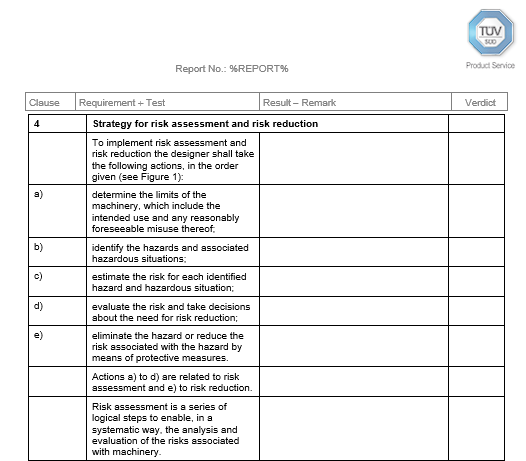
\includegraphics[width=\textwidth]{img/trf.png}

\bigskip \adjustimage{width=\textwidth, center, caption={Test Report Form}, label={fig1}, nofloat=figure, vspace=\bigskipamount}{img/trf.png}

\paragraph{} A more recent approach to risk assessment might be the use of mCom ONE which is being used currently. mCom ONE is a cloud based software solution that facilitates life-cycle management of hazards by bringing machinery, people and processes together while keeping the data readily available for stakeholders across sites \cite{mcom}. mCom ONE provides a centralized platform that allows companies to manage and track their regulatory compliance requirements, including product safety testing and certification, regulatory reporting, and quality control. The platform also provides real-time visibility into compliance status and allows for proactive identification of potential compliance issues. This tool supports engineer in following a checklist based audit to identify hazards according to safety standards. The workflow remains the same instead the TRF is now replaced by its digital counterpart. 

% \bigskip 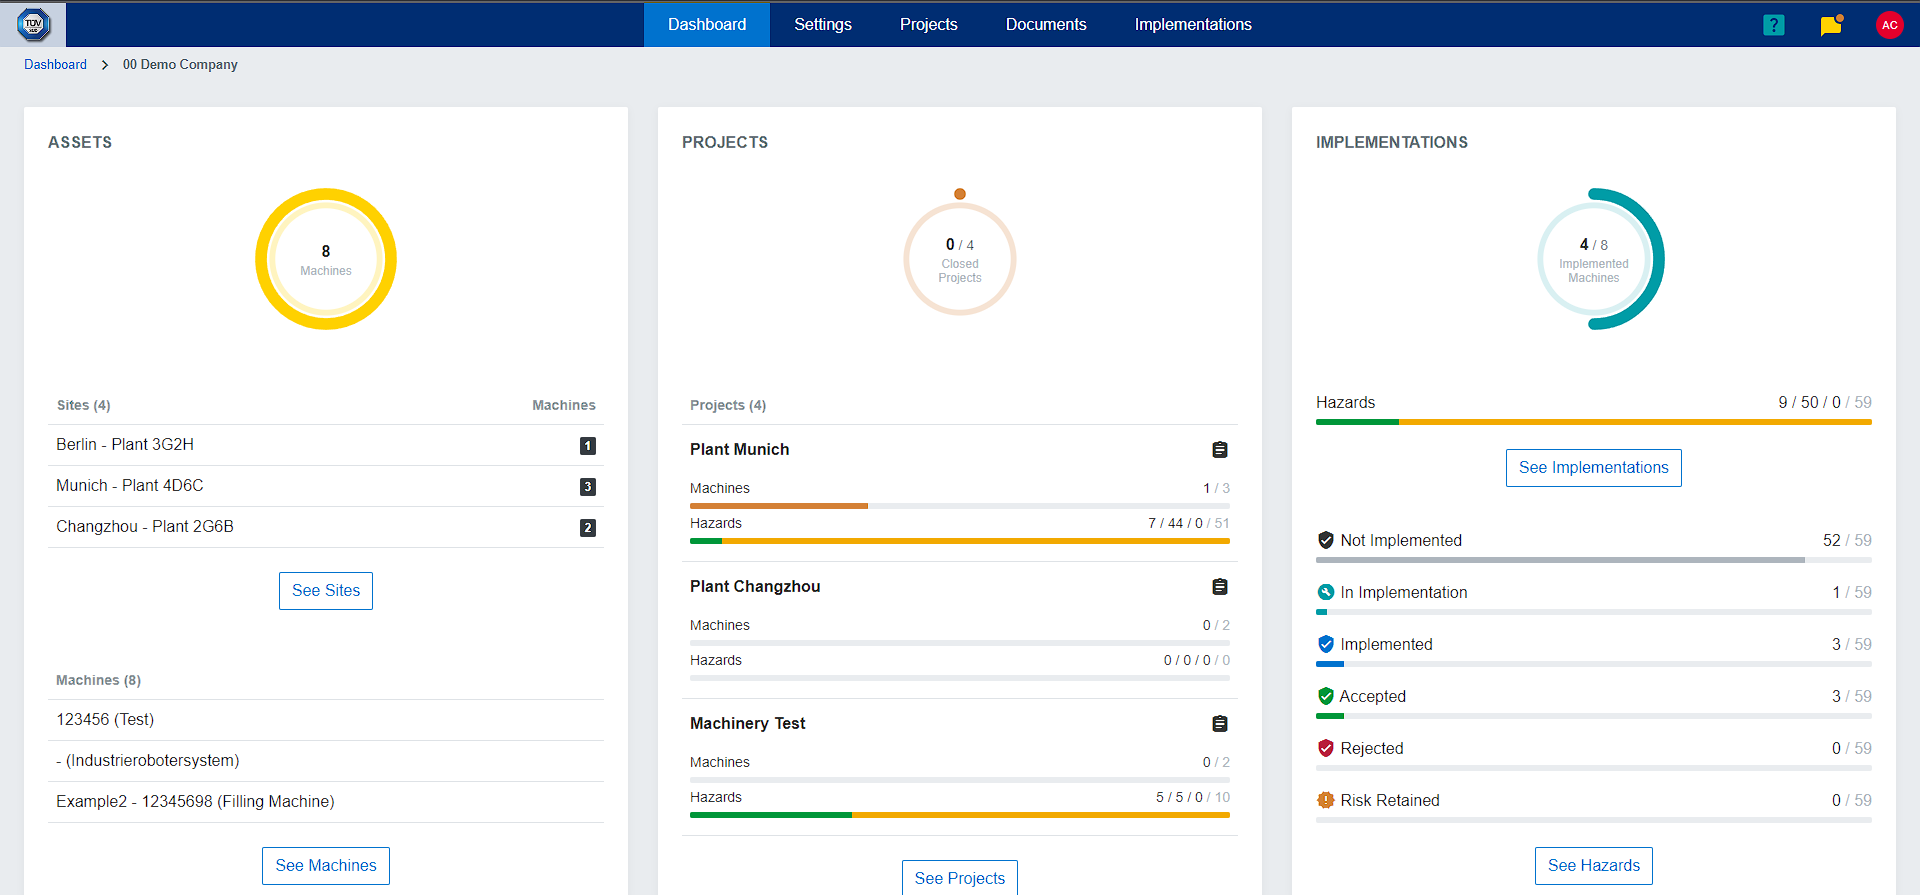
\includegraphics[width=\textwidth]{img/mCom.png}

\bigskip \adjustimage{width=\textwidth, center, caption={mCom ONE dashboard}, label={fig2}, nofloat=figure, vspace=\bigskipamount}{img/mCom.png}

\section{Knowledge model}\label{km}
A knowledge model is a representation of knowledge that captures the concepts and relationships of a specific domain. It is a structured and formal representation of knowledge that can be used to support decision-making, problem-solving, and knowledge management in various applications. As surveyed by Yun et al. \cite{Yun2021}, a knowledge model can be represented in various forms such as semantic networks, ontologies, decision trees, and rule-based systems. It can be used to capture knowledge from experts and documents in a particular field or domain, and then codify and organize that knowledge in a way that can be shared and reused by others.

\paragraph{} A knowledge model can be used in a wide range of applications such as artificial intelligence, knowledge management, and expert systems. In artificial intelligence, knowledge models can be used to represent knowledge in a specific domain to support reasoning and decision-making. In knowledge management, knowledge models can be used to organize and manage knowledge in a particular organization or community. In expert systems, knowledge models can be used to capture the knowledge of experts and automate decision-making processes.

\subsection{How to model knowledge} \label{how_to_model}
According to the studies by Dong et al. \cite{Dong2022} and Yun et al. \cite{Yun2021}, there are many ways to model knowledge, depending on the type and complexity of the knowledge to be represented. Some common approaches to modeling knowledge include:

\begin{itemize}
    \item \textbf{Ontologies:} An ontology is a formal representation of a domain of knowledge that defines the concepts and relationships within that domain. Ontologies are often used to represent complex or specialized knowledge and can be used in applications such as natural language processing and artificial intelligence.
    \item \textbf{Concept maps:}  A concept map is a graphical representation of a domain of knowledge that shows the relationships between different concepts. Concept maps can be used to visualize and organize knowledge, as well as to identify gaps or inconsistencies in the knowledge.
    \item \textbf{Knowledge graphs:}  A knowledge graph is a graph-based representation of structured knowledge that consists of entities (also known as nodes or vertices) and the relationships between them (also known as edges or arcs). Knowledge graphs are often used to represent and organize knowledge in a machine-readable format, and are used in applications such as search engines and recommendation systems.
    \item \textbf{Semantic networks:}  A semantic network is a graphical representation of the meaning of words or concepts in a domain of knowledge. Semantic networks can be used to represent the relationships between different concepts and to understand the meaning of words or phrases in context.
    \item \textbf{Decision trees:}  A decision tree is a graphical representation of a decision-making process that shows the possible outcomes of a series of decisions. Decision trees can be used to model knowledge about decision-making processes and to make predictions or recommendations based on that knowledge.
\end{itemize}

 \subsection{Knowledge modeling in industrial risk assessments} \label{km_in_ira}
 Knowledge models can be used to make industrial risk assessment more efficient by providing a structured representation of the knowledge and information relevant to the risk assessment process. For example, an ontology or a knowledge graph can be used to represent the concepts and relationships related to the industrial processes being studied, the hazards associated with those processes, and the control measures that can be implemented to mitigate those hazards. This structured representation of knowledge can then be used to automate parts of the risk assessment process, such as identifying relevant hazards or control measures, or to support decision-making by providing relevant information at the appropriate stage of the process. Knowledge models can also be used to support the continuous improvement of the risk assessment process by providing a framework for organizing and storing information about past risk assessments, identifying trends and patterns in the data, and tracking the effectiveness of risk control measures over time.
 
 \paragraph{} A knowledge model for industrial risk assessment may include information about the types of hazards associated with different industrial processes, such as mechanical, electrical, vibration, noise, radiation and multiple other hazards. It may also include information about risk reduction measures, preventive measures, testing requirements, that can be used to mitigate these hazards. In addition, a knowledge model for industrial risk assessment may include information about regulations and standards related to industrial safety, such as ISO 12100 and other relevant safety standards. This information can help ensure that risk assessments are conducted in compliance with applicable regulations and standards. 